% Options for packages loaded elsewhere
\PassOptionsToPackage{unicode}{hyperref}
\PassOptionsToPackage{hyphens}{url}
%
\documentclass[
]{article}
\usepackage{amsmath,amssymb}
\usepackage{lmodern}
\usepackage{ifxetex,ifluatex}
\ifnum 0\ifxetex 1\fi\ifluatex 1\fi=0 % if pdftex
  \usepackage[T1]{fontenc}
  \usepackage[utf8]{inputenc}
  \usepackage{textcomp} % provide euro and other symbols
\else % if luatex or xetex
  \usepackage{unicode-math}
  \defaultfontfeatures{Scale=MatchLowercase}
  \defaultfontfeatures[\rmfamily]{Ligatures=TeX,Scale=1}
\fi
% Use upquote if available, for straight quotes in verbatim environments
\IfFileExists{upquote.sty}{\usepackage{upquote}}{}
\IfFileExists{microtype.sty}{% use microtype if available
  \usepackage[]{microtype}
  \UseMicrotypeSet[protrusion]{basicmath} % disable protrusion for tt fonts
}{}
\makeatletter
\@ifundefined{KOMAClassName}{% if non-KOMA class
  \IfFileExists{parskip.sty}{%
    \usepackage{parskip}
  }{% else
    \setlength{\parindent}{0pt}
    \setlength{\parskip}{6pt plus 2pt minus 1pt}}
}{% if KOMA class
  \KOMAoptions{parskip=half}}
\makeatother
\usepackage{xcolor}
\IfFileExists{xurl.sty}{\usepackage{xurl}}{} % add URL line breaks if available
\IfFileExists{bookmark.sty}{\usepackage{bookmark}}{\usepackage{hyperref}}
\hypersetup{
  pdftitle={SimplyAgree: An R package and jamovi Module for Simplifying Agreement and Reliability Analyses},
  hidelinks,
  pdfcreator={LaTeX via pandoc}}
\urlstyle{same} % disable monospaced font for URLs
\usepackage[margin=1in]{geometry}
\usepackage{graphicx}
\makeatletter
\def\maxwidth{\ifdim\Gin@nat@width>\linewidth\linewidth\else\Gin@nat@width\fi}
\def\maxheight{\ifdim\Gin@nat@height>\textheight\textheight\else\Gin@nat@height\fi}
\makeatother
% Scale images if necessary, so that they will not overflow the page
% margins by default, and it is still possible to overwrite the defaults
% using explicit options in \includegraphics[width, height, ...]{}
\setkeys{Gin}{width=\maxwidth,height=\maxheight,keepaspectratio}
% Set default figure placement to htbp
\makeatletter
\def\fps@figure{htbp}
\makeatother
\setlength{\emergencystretch}{3em} % prevent overfull lines
\providecommand{\tightlist}{%
  \setlength{\itemsep}{0pt}\setlength{\parskip}{0pt}}
\setcounter{secnumdepth}{-\maxdimen} % remove section numbering
\ifluatex
  \usepackage{selnolig}  % disable illegal ligatures
\fi
\newlength{\cslhangindent}
\setlength{\cslhangindent}{1.5em}
\newlength{\csllabelwidth}
\setlength{\csllabelwidth}{3em}
\newenvironment{CSLReferences}[2] % #1 hanging-ident, #2 entry spacing
 {% don't indent paragraphs
  \setlength{\parindent}{0pt}
  % turn on hanging indent if param 1 is 1
  \ifodd #1 \everypar{\setlength{\hangindent}{\cslhangindent}}\ignorespaces\fi
  % set entry spacing
  \ifnum #2 > 0
  \setlength{\parskip}{#2\baselineskip}
  \fi
 }%
 {}
\usepackage{calc}
\newcommand{\CSLBlock}[1]{#1\hfill\break}
\newcommand{\CSLLeftMargin}[1]{\parbox[t]{\csllabelwidth}{#1}}
\newcommand{\CSLRightInline}[1]{\parbox[t]{\linewidth - \csllabelwidth}{#1}\break}
\newcommand{\CSLIndent}[1]{\hspace{\cslhangindent}#1}

\title{SimplyAgree: An R package and jamovi Module for Simplifying
Agreement and Reliability Analyses}
\author{}
\date{\vspace{-2.5em}}

\begin{document}
\maketitle

\hypertarget{summary}{%
\section{Summary}\label{summary}}

Accurate and reliable measurements are critical to quantitative research
efforts. Based on citation counts, researchers highly value methods to
quantify the accuracy and reliability of the measurement tools (J.
Martin Bland \& Altman, 1986; Weir, 2005). This article introduces the
\texttt{SimplyAgree} R package and jamovi module as user-friendly
solutions for estimating agreement and reliability (R Core Team, 2020;
The jamovi project, 2021). Updates and additional details on
\texttt{SimplyAgree}

\hypertarget{statement-of-need}{%
\section{Statement of Need}\label{statement-of-need}}

A number of new methods have been developed in the past three decades to
improve the calculation of the limits of agreement (Lin, 1989; Shieh,
2019; Zou, 2011) and other measures of measurement reliability
(Carrasco, Phillips, Puig-Martinez, King, \& Chinchilli, 2013; Weir,
2005). However, to author's best knowledge, statistical software ---
particularly open source software --- to implement these statistical
analyses is lacking. While some software may provide the limits of
agreement analysis outlined by Bland \& Altman (1999; 1986), few, if
any, account for multiple observations within the same research subject
(Zou, 2011) or include hypothesis tests of agreement (Shieh, 2019). Many
researchers may not have the skills necessary to write the code, from
scratch, in order to implement many of the newest techniques. The jamovi
project (2021) is a open source statistical platform that provides a
graphical user interface (GUI), and therefore is an accessible source
for researchers without coding experience. Therefore, a jamovi module of
\texttt{SimplyAgree} was also created in order to reach those
researchers who may not have the coding expertise required to
effectively use the R package.

\hypertarget{current-r-capabilities}{%
\section{Current R Capabilities}\label{current-r-capabilities}}

The R package \texttt{SimplyAgree}, currently v0.0.2 on the
comprehensive R archive network (CRAN), implements a number of useful
agreement and reliability analyses.

The current release of the R package can be downloaded directly from
CRAN in R:

\begin{verbatim}
install.packages("SimplyAgree")
\end{verbatim}

Or, the developmental version, can be downloaded from GitHub:

\begin{verbatim}
devtools::install_github("arcaldwell49/SimplyAgree")
\end{verbatim}

There are 2 vignettes that document the major functions within the
package that can be found on the package's website
(\url{https://aaroncaldwell.us/SimplyAgree}). Overall, there are 6
fundamental functions, all with generic \texttt{plot} and \texttt{print}
methods, within the R package:

\begin{enumerate}
\def\labelenumi{\arabic{enumi}.}
\item
  \texttt{agree\_test}: Simple Test of Agreement. This is function
  performs agreement analyses on two vectors of the same length, and is
  designed for analyses that were described by Bland \& Altman (1999;
  1986). In addition to providing the traditional Bland-Altman limits of
  agreement, the function provides a hypothesis test (Shieh, 2019), and
  provides the concordance correlation coefficient (Lin, 1989).
\item
  \texttt{agree\_reps}: Test of Agreement for Replicate Data. This
  function provides the limits of agreement described by Zou (2011) for
  data where the mean, per subject, does not vary. In addition, the
  concordance correlation coefficient, calculated by U-statistics, is
  also provided in the output (Carrasco, Phillips, Puig-Martinez, King,
  \& Chinchilli, 2013).
\item
  \texttt{agree\_nest}: Test of Agreement for Nested Data. This function
  provides the limits of agreement described by Zou (2011) for data
  where the mean, per subject, \emph{does} vary. Similar to the
  replicate data function, the concordance correlation coefficient,
  calculated by U-statistics, is provided in the output (Carrasco,
  Phillips, Puig-Martinez, King, \& Chinchilli, 2013).
\item
  \texttt{loa\_mixed}: Bootstrapped Limits of Agreement for Nested Data.
  This function calculates limits of agreement using a non-parametric
  bootstrap method, and can allow the underlying mean to vary (replicate
  data) or not (nested data).
\item
  \texttt{blandPowerCurve}: Power Analysis for Bland-Altman Limits of
  Agreement. This function implements the formula outlined by Lu et al.
  (2016). This allows for power calculations for the J. Martin Bland \&
  Altman (1999) limits of agreement. The function \texttt{find\_n} can
  then be used to find the sample size at which adequate power (defined
  by the user) is achieved.
\item
  \texttt{reli\_stats}: Reliability Statistics. This function calculates
  and provides as output the statistics outlined by Weir (2005). This
  includes an array of intraclass correlation coefficients, the
  coefficient of variation, and the standard error of measurement.
\end{enumerate}

\hypertarget{current-jamovi-capabilities}{%
\section{Current jamovi
Capabilities}\label{current-jamovi-capabilities}}

The jamovi module can be added to the jamovi directly from the ``add
module'' tab in the GUI.

\begin{figure}
\centering
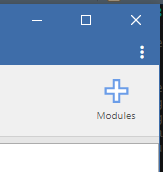
\includegraphics{module_button.PNG}
\caption{\textbf{Figure 1}: How to add a module in jamovi.}
\end{figure}

The \texttt{SimplyAgree} module is then available on the main menu, and
within it there are three analysis options.

\begin{figure}
\centering
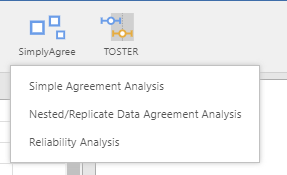
\includegraphics{simplyagree_button.PNG}
\caption{\textbf{Figure 2}: SimplyAgree in jamovi.}
\end{figure}

The three analysis options essentially enable jamovi users to complete
some of the same analyses available in the R package.

\begin{enumerate}
\def\labelenumi{\arabic{enumi}.}
\tightlist
\item
  The simple agreement analysis incorporates the \texttt{agree\_test}
  function. Users have the option of including the concordance
  correlation coefficient, and plots of the data.
\end{enumerate}

\begin{figure}
\centering
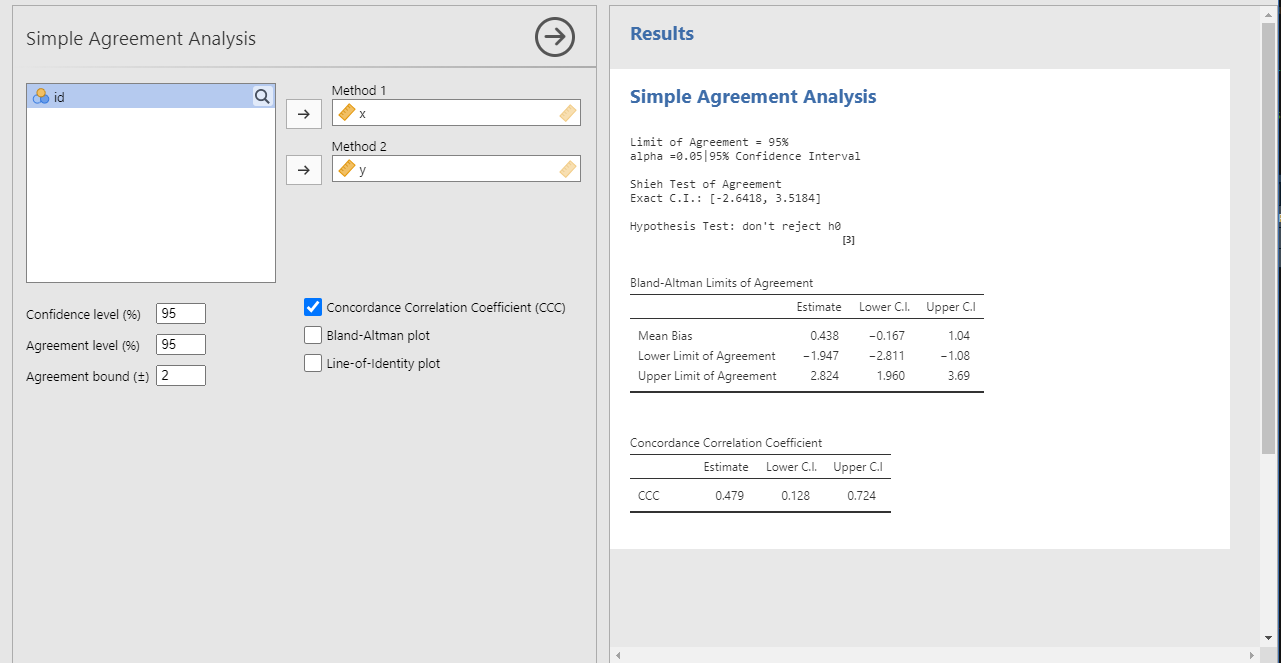
\includegraphics{simple_agreement.PNG}
\caption{\textbf{Figure 3}: Sample Output from the Simple Agreement
Analysis.}
\end{figure}

\begin{enumerate}
\def\labelenumi{\arabic{enumi}.}
\setcounter{enumi}{1}
\tightlist
\item
  The nested/replicate agreement analysis uses the \texttt{agree\_nest}
  and \texttt{agree\_reps} function to perform the analyses. The
  \texttt{agree\_reps} function is used if ``Assume underlying value
  does not vary?'' is selected; otherwise \texttt{agree\_nest} is used.
\end{enumerate}

\begin{figure}
\centering
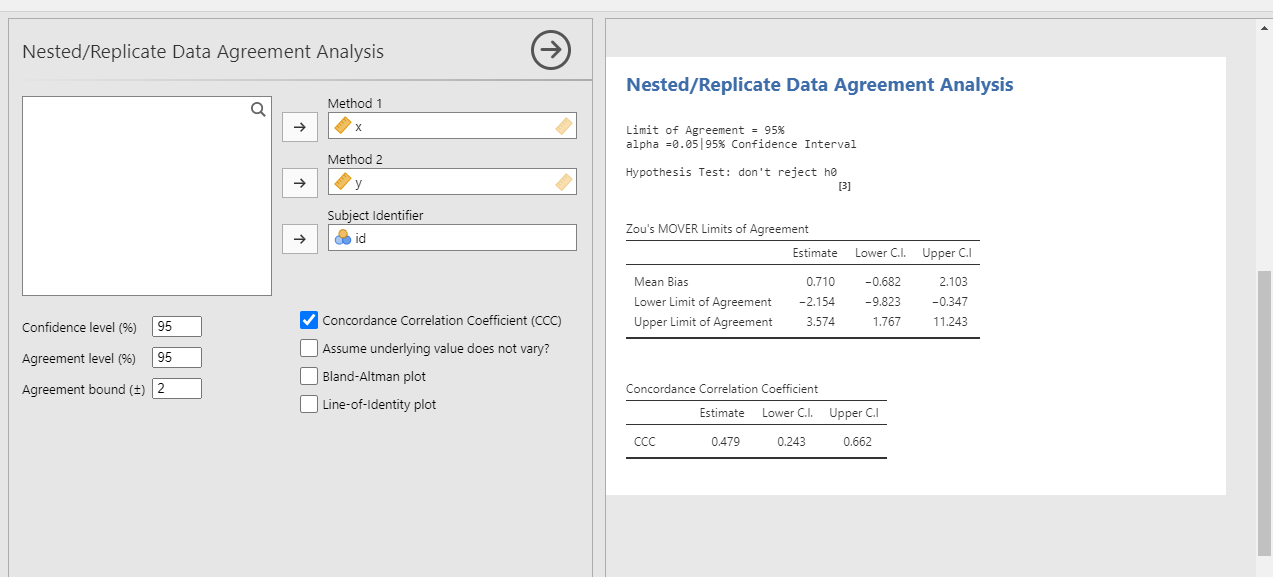
\includegraphics{nested_agreement.PNG}
\caption{\textbf{Figure 4}:Sample Output from the Nested/Replicate
Agreement Analysis.}
\end{figure}

\begin{enumerate}
\def\labelenumi{\arabic{enumi}.}
\setcounter{enumi}{2}
\tightlist
\item
  The reliability analysis utilizes \texttt{reli\_stats} to calculate
  reliability statistics.
\end{enumerate}

\begin{figure}
\centering
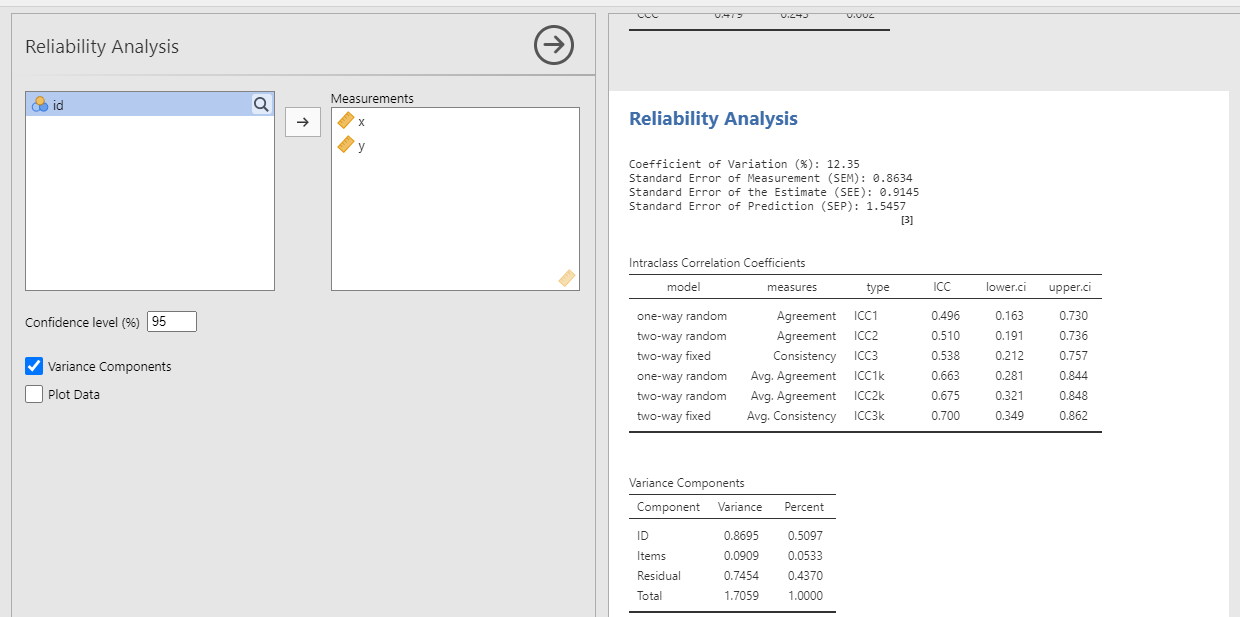
\includegraphics{reliability.PNG}
\caption{\textbf{Figure 5}: Sample Output from the Reliability
Analsyis.}
\end{figure}

\hypertarget{acknowledgements}{%
\section{Acknowledgements}\label{acknowledgements}}

I would like the thank Ashley Akerman for his kind feedback during the
development of this package.

The opinions or assertions contained herein are the private views of the
author and are not to be construed as official or reflecting the views
of the Army or the Department of Defense. Any citations of commercial
organizations and trade names in this report do not constitute an
official Department of the Army endorsement of approval of the products
or services of these organizations. No authors have any conflicts of
interest to disclose. Approved for public release; distribution is
unlimited.

\hypertarget{references}{%
\section*{References}\label{references}}
\addcontentsline{toc}{section}{References}

\hypertarget{refs}{}
\begin{CSLReferences}{1}{0}
\leavevmode\hypertarget{ref-bland1999}{}%
Bland, J. Martin, \& Altman, D. G. (1999). Measuring agreement in method
comparison studies. \emph{Statistical Methods in Medical Research},
\emph{8}(2), 135--160.
doi:\href{https://doi.org/10.1177/096228029900800204}{10.1177/096228029900800204}

\leavevmode\hypertarget{ref-bland1986}{}%
Bland, J. Martin, \& Altman, DouglasG. (1986). Statistical methods for
assessing agreement between two methods of clinical measurement.
\emph{The Lancet}, \emph{327}(8476), 307--310.
doi:\href{https://doi.org/10.1016/s0140-6736(86)90837-8}{10.1016/s0140-6736(86)90837-8}

\leavevmode\hypertarget{ref-carrasco2013}{}%
Carrasco, J. L., Phillips, B. R., Puig-Martinez, J., King, T. S., \&
Chinchilli, V. M. (2013). Estimation of the concordance correlation
coefficient for repeated measures using {SAS} and r. \emph{Computer
Methods and Programs in Biomedicine}, \emph{109}(3), 293--304.
doi:\href{https://doi.org/10.1016/j.cmpb.2012.09.002}{10.1016/j.cmpb.2012.09.002}

\leavevmode\hypertarget{ref-lin1989}{}%
Lin, L. I.-K. (1989). A concordance correlation coefficient to evaluate
reproducibility. \emph{Biometrics}, \emph{45}(1), 255.
doi:\href{https://doi.org/10.2307/2532051}{10.2307/2532051}

\leavevmode\hypertarget{ref-lu2016}{}%
Lu, M.-J., Zhong, W.-H., Liu, Y.-X., Miao, H.-Z., Li, Y.-C., \& Ji,
M.-H. (2016). Sample size for assessing agreement between two methods of
measurement by bland-altman method. \emph{The International Journal of
Biostatistics}, \emph{12}(2).
doi:\href{https://doi.org/10.1515/ijb-2015-0039}{10.1515/ijb-2015-0039}

\leavevmode\hypertarget{ref-R-base}{}%
R Core Team. (2020). \emph{R: A language and environment for statistical
computing}. Vienna, Austria: R Foundation for Statistical Computing.
Retrieved from \url{https://www.R-project.org/}

\leavevmode\hypertarget{ref-shieh2019}{}%
Shieh, G. (2019). Assessing agreement between two methods of
quantitative measurements: Exact test procedure and sample size
calculation. \emph{Statistics in Biopharmaceutical Research},
\emph{12}(3), 352--359.
doi:\href{https://doi.org/10.1080/19466315.2019.1677495}{10.1080/19466315.2019.1677495}

\leavevmode\hypertarget{ref-jamovi}{}%
The jamovi project. (2021). \emph{Jamovi}. Retrieved from
\url{https://www.jamovi.org}

\leavevmode\hypertarget{ref-weir2005}{}%
Weir, J. P. (2005). Quantifying test-retest reliability using the
intraclass correlation coefficient and the {SEM}. \emph{The Journal of
Strength and Conditioning Research}, \emph{19}(1), 231. Retrieved from
\url{https://pubmed.ncbi.nlm.nih.gov/15705040/}

\leavevmode\hypertarget{ref-zou2011}{}%
Zou, G. (2011). Confidence interval estimation for the bland{{}}altman
limits of agreement with multiple observations per individual.
\emph{Statistical Methods in Medical Research}, \emph{22}(6), 630--642.
doi:\href{https://doi.org/10.1177/0962280211402548}{10.1177/0962280211402548}

\end{CSLReferences}

\end{document}
